\documentclass[11pt,a4paper]{article}
\usepackage{fontspec}
\setmainfont{TeX Gyre Pagella}
\newfontfamily\headfont{Inter}[UprightFont=*-ExtraBold,BoldFont=*-ExtraBold,Extension=.otf,Path=/usr/share/fonts/opentype/inter/]
\usepackage[a4paper,margin=2.3cm]{geometry}
\usepackage{graphicx,booktabs,float,caption,array,xcolor,amsmath}
\usepackage{xurl}
\usepackage[hidelinks]{hyperref}
\usepackage{titlesec}
\usepackage{setspace}
\usepackage[round]{natbib}
\setstretch{1.05}
\renewcommand{\topfraction}{0.9}
\renewcommand{\bottomfraction}{0.8}
\renewcommand{\textfraction}{0.1}
\renewcommand{\floatpagefraction}{0.75}
\setlength{\parindent}{0pt}
\setlength{\parskip}{0.55em}
\titleformat{\section}{\headfont\Large}{\thesection}{0.8em}{}
\titleformat{\subsection}{\headfont\large}{\thesubsection}{0.8em}{}
\captionsetup{font=small,labelfont=bf}
\urlstyle{same}
\hypersetup{pdftitle={The Inked World},pdfauthor={Tristan Hotham}}

\begin{document}
\begin{center}
{\Large\bfseries The Inked World\par}
\vspace{0.4em}
{\large A Tolkien-inspired map of the modern Earth: a zoomable world map\\in the style of a hand-inked fantasy map, generated from open data\par}
\vspace{1.2em}
{\large Tristan Hotham\par}
\vspace{0.3em}
{\small Independent researcher\\
ORCID: 0000-0003-4931-9349\\
DOI: \url{https://doi.org/10.5281/zenodo.23860253}\par}
\vspace{0.8em}
2026
\end{center}

\begin{quote}
\small
\begin{center}\textbf{Abstract}\end{center}
I describe a Tolkien-inspired map of the modern Earth. Hand-drawn maps, with rows of inked mountains, clusters of tiny trees, coasts traced with thin parallel lines and names lettered in red, are made for one place at one scale. This is a zoomable map of the whole world in that style, generated in the reader's browser from open data: OpenStreetMap vector tiles from OpenFreeMap and the AWS Terrain Tiles elevation model. Mountains and hills are placed on the highest points of a nested grid of cells, where the relief clears a bar that grows with the size of the cell on the ground, from about 477~m for cells of 237~km at zoom 2 to about 130~m for cells of 311~m at zoom 11. Because the highest point of a cell is also the highest point of one of its children, peaks persist as one zooms in and new ones fade in between them. A spacing rule keeps glyphs off plain slopes, a ruggedness test keeps peaks off high flat plateaus and deserts, and a thinning rule keeps great ranges readable. Between the ranges, dunes, grass, rainforest, taiga and ice glyphs follow the RESOLVE Ecoregions biomes; trees fill OpenStreetMap woods, nothing is drawn on water, and names are placed before glyphs: 194 countries along fitted or hand-drawn curves, and 167 hand-placed oceans, seas, ranges, deserts and regions, cut to fit their text at every zoom. Heritage sites from Wikidata appear as small drawings ranked by their Wikipedia coverage, towns fill with houses along their real streets close in, peaks above the snow line carry snow, and animals, whales and sailing ships decorate the map in their real ranges and lanes. Every visual parameter is interpolated over zoom, so the map reads as one drawing from the globe to a single hill. I set out the rules, show the result from the world to the Lake District, and discuss the limits.

\textbf{Keywords:} Tolkien-inspired map; fantasy cartography; hand-drawn map style; cartography; generative maps; fantasy maps; OpenStreetMap; digital elevation models; MapLibre; label placement; level of detail; open data
\end{quote}

\section{Introduction}
The maps at the front of fantasy novels, and many older printed maps, share a look that most readers recognise at once: mountains drawn as rows of small inked peaks, forests as clusters of tiny trees, coasts traced with several thin parallel lines, and names lettered by hand in red across the land and sea. That look depends on a map maker's judgement about what to draw where, and it is made for one place at one scale. Interactive web maps go the other way: they can show anywhere at any scale, but in a uniform, modern style.

This paper describes a map that tries to have both. The Inked World is a zoomable map of the whole world, available at \url{https://maps.tristanhotham.com/ink-map/}, that draws itself in a hand-inked style at every zoom, from the whole globe down to a single hill, using only open data: OpenStreetMap vector tiles served by OpenFreeMap, and the AWS Terrain Tiles elevation model. Nothing is traced from an existing drawing. Every mountain glyph is placed by a rule applied to elevation, every tree by a rule applied to mapped woodland, and every name either comes from OpenStreetMap or is lettered along a curve that I drew for it. The map was inspired by the general look of hand-drawn maps, Tolkien's among them, but no artwork, lettering, cartouche or emblem from any map was copied, and it is not connected with or endorsed by the Tolkien Estate.

Three design goals shaped it. First, it should look drawn, not rendered: black ink for coasts and relief, red for names, blue for water, on parchment. Second, it should change smoothly with zoom: zooming in should add detail to the same drawing rather than switch from one style to another. Third, it should work for the whole world, live, with no tiles to pre-render or host. The rest of the paper sets out the data (Section~2), the rules (Section~3), what the map looks like and how it was checked (Sections~4 and~5), and its limits (Section~6).

\section{Data}
\textbf{OpenStreetMap.} All land, water, rivers, place names, peaks, roads, borders and land cover come from OpenStreetMap \citep{osm}, as vector tiles built by OpenFreeMap \citep{openfreemap} in the OpenMapTiles schema \citep{openmaptiles}. The map uses the \texttt{water}, \texttt{waterway}, \texttt{landcover}, \texttt{place}, \texttt{mountain\_peak}, \texttt{boundary}, \texttt{transportation}, \texttt{water\_name} and \texttt{park} layers. The data are under the Open Database Licence and are read live by the page; no tile data are redistributed.

\textbf{Elevation.} The AWS Terrain Tiles \citep{terrain} are a global elevation model in web map tiles, built by Mapzen from SRTM, GMTED2010, ETOPO1 and national models. The map reads the Terrarium encoding, in which each pixel's red, green and blue values give the elevation in metres as $256R + G + B/256 - 32768$.

\textbf{Biomes.} RESOLVE Ecoregions 2017 \citep{resolve} divides the land into 846 ecoregions in 14 biomes, plus rock and ice, under CC BY 4.0. I read a copy simplified at 0.005 degrees and rasterise it to a 2048 pixel web Mercator mask of seven classes: desert (sandy and true deserts, by name; shrub steppes and xeric scrub join the grassland class); grassland, savanna and steppe (tropical, temperate and montane grasslands); tropical moist forest; boreal forest; ice; flooded grassland; tundra. Temperate and Mediterranean forests get no biome glyphs. 181 ecoregions whose names refer to mountains (for example \emph{Mediterranean High Atlas juniper steppe} or \emph{Tibesti-Jebel Uweinat montane xeric woodlands}) are flagged, except plateaus.

\textbf{Outlines for lettering.} Country names are lettered along curves fitted to Natural Earth's 1:50m country outlines \citep{naturalearth}; the four nations of the United Kingdom along curves fitted to the Office for National Statistics' local authority district boundaries \citep{ons}. Search uses Natural Earth's populated places and states and provinces.

\textbf{Fonts.} MedievalSharp for capitals, and IM Fell English, IM Fell English Small Caps and IM Fell Great Primer Italic for everything else \citep{fonts}, all under the SIL Open Font License, converted to the signed distance field glyphs MapLibre needs with fontnik.

\section{Method}
\subsection{Architecture}
The page is a static file using MapLibre GL JS \citep{maplibre}. Most of the map is an ordinary vector style over the OpenFreeMap tiles. The hand-drawn elements, mountains, hills, trees and tufts of marsh and moor, are not in any tile set, so the page registers a custom tile protocol, \texttt{ink://}, served by a small pool of web workers. For each requested tile the worker fetches the elevation tiles and the OpenStreetMap tile for the same area, computes where glyphs go, and returns a vector tile of points. MapLibre then draws those points with glyph images that the page paints on canvas when it loads (Figure~\ref{fig:glyphs}). Because everything is computed in the reader's browser from live tiles, the whole world works at every zoom with nothing to pre-render or host.

\begin{figure}[tbp]\centering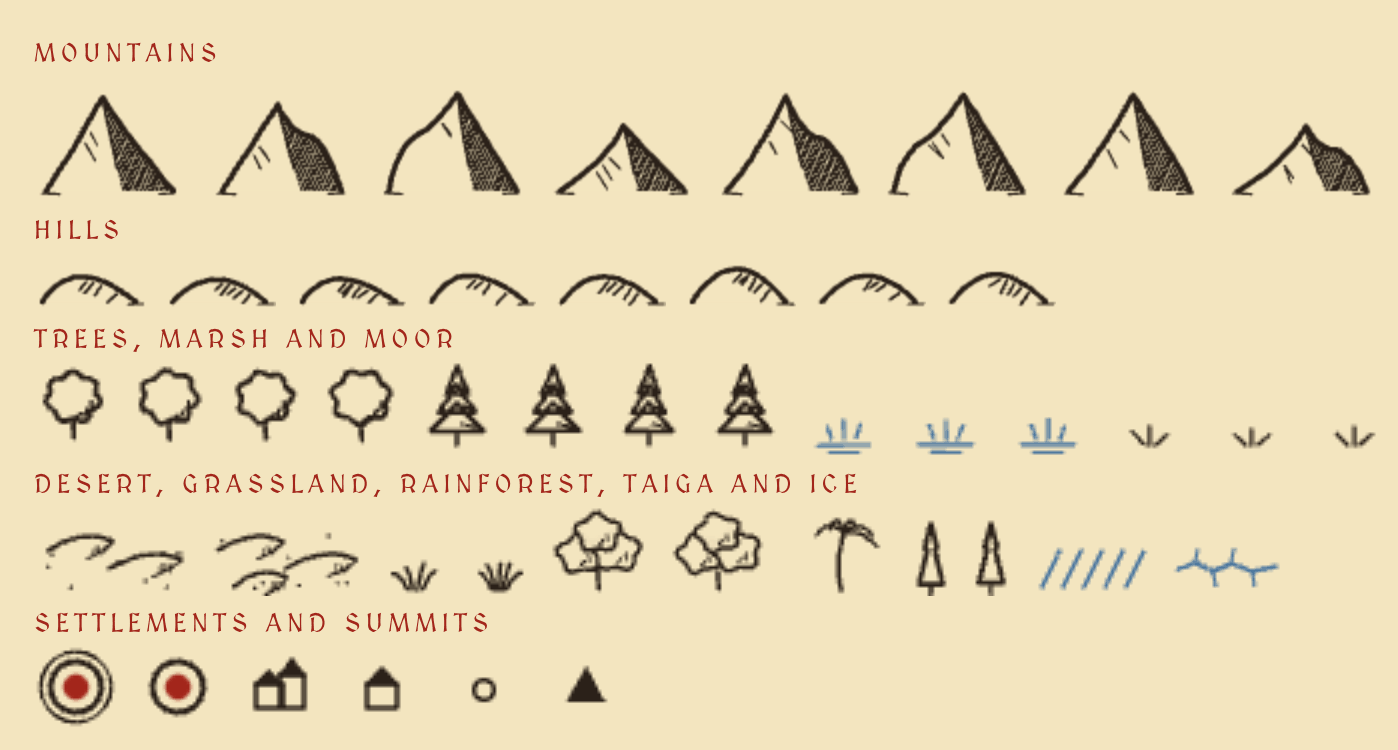
\includegraphics[width=0.92\textwidth]{f_glyphs.png}
\caption{The glyphs, drawn on canvas by the page: eight mountains, eight hills, broadleaf and conifer trees, marsh and moor tufts, biome glyphs, and a selection of the pictograms for settlements, snow, heritage, famous monuments, animals, ships and flight. Each is drawn with a slight random wobble, so no two strokes are perfectly straight.}\label{fig:glyphs}\end{figure}

\subsection{Mountains and hills}
The worker lays a grid over the map whose cells are 14 screen pixels across at the zoom where they first appear: a cell of rank $r$ has side $c_r = 14/(512 \cdot 2^r)$ in normalised web Mercator units, so each cell splits into four at the next rank. For every cell it finds the highest point and the elevation $h$ there, and the lowest elevation $\ell$ in the $3\times 3$ block of cells around it (never below sea level). The relief $h - \ell$ is compared with a threshold that grows with the size of the cell on the ground, $s$ in kilometres:
\[ T = A \, s^{0.3} \, f_d, \qquad A = 185~\text{m}, \]
where $f_d$ is a correction for the resolution $d$ of the elevation tiles: far out the tiles are coarse and smooth the summits down, so the bar is lowered ($f_d = 0.5$ for $d \le 4$, $0.68$ for $d \le 6$, $0.85$ for $d \le 8$, $1$ beyond). A point with relief of at least $T$ gets a mountain; one with at least $40\%$ of $T$ a rounded hill; anything less, nothing. Table~\ref{tab:thresholds} gives the bar at each rank. Glyph size grows with relief over threshold, and glyphs are drawn back to front so that nearer peaks overlap farther ones.

\begin{table}[tbp]\centering\small\caption{Relief needed for a mountain and a hill, by rank (the zoom at which a cell is 14 screen pixels across), for a cell at latitude 45 degrees.}\label{tab:thresholds}\begin{tabular}{rrrr}\toprule Rank & Cell (km) & Mountain (m) & Hill (m)\\\midrule
1 & 387.42 & 553 & 221\\
2 & 193.71 & 449 & 180\\
3 & 96.86 & 365 & 146\\
4 & 48.43 & 403 & 161\\
5 & 24.21 & 327 & 131\\
6 & 12.11 & 332 & 133\\
7 & 6.05 & 270 & 108\\
8 & 3.03 & 258 & 103\\
9 & 1.51 & 209 & 84\\
10 & 0.76 & 170 & 68\\
11 & 0.38 & 138 & 55\\
12 & 0.19 & 112 & 45\\
\bottomrule\end{tabular}\end{table}

Relief alone puts peaks on high flat ground: a plateau edge, or a broad desert upland seen through coarse tiles, can rise hundreds of metres above the lowest cell nearby. So a candidate must also be rugged. The worker accumulates the absolute elevation change between neighbouring pixels in every cell and takes the mean slope, in metres per kilometre, over the $3\times3$ finest cells around the candidate's highest point. A mountain needs a slope of at least $G_d$, which rises with the elevation zoom $d$ because finer tiles reveal steeper slopes (4, 4.5, 5.5, 7.5, 10, 12, 13, 22, 30, 38, 48, 60, 70 for $d = 0$ to 12); a hill needs 45\% of that. In flagged montane ecoregions the bar is multiplied by 0.3, so that narrow ranges such as the Atlas or the Ahaggar, smoothed on coarse tiles, still count; in desert, grassland, rainforest, taiga and tundra ecoregions without the flag it is multiplied by 1.5, so that dissected plateaus become hills. On ice, hills are dropped: the edge of an ice sheet is not a hill.

Two further rules keep the glyphs on summits and ridges. A point is dropped when a neighbouring cell's higher point lies within a fraction of a cell width of it (0.55 of a cell for cells over a kilometre across, rising to a whole cell for cells of 100~m); on an even slope, every cell's highest point lies on its uphill edge, and without this rule the glyphs would run in rows down the hillside (Figure~\ref{fig:method}). And in a great range, where every cell clears the bar by a wide margin, a mountain is left out when at least 6 of its eight neighbours are mountains, at least 3 of those are higher, and the mean relief around it is at least 2.2 times the bar, for cells under 10~km (one more higher neighbour is needed for cells of 10 to 30~km, and the rule is off beyond). This keeps the ridges and summits of the Himalaya or the Alps readable, rather than a solid mass of ink, and almost never applies in hill country such as the Lake District. No new ranks are added beyond rank 12, where a cell is about 190~m across and would measure the slope of a hillside rather than a summit.

The important property is nesting. The highest point of a cell is also the highest point of one of its four children, so a peak placed at one rank is a candidate at every finer rank. Each tile computes three consecutive ranks and the style fades each rank in over the zoom before its own, so zooming in adds new, smaller peaks between the old ones without moving or removing them.

\begin{figure}[tbp]\centering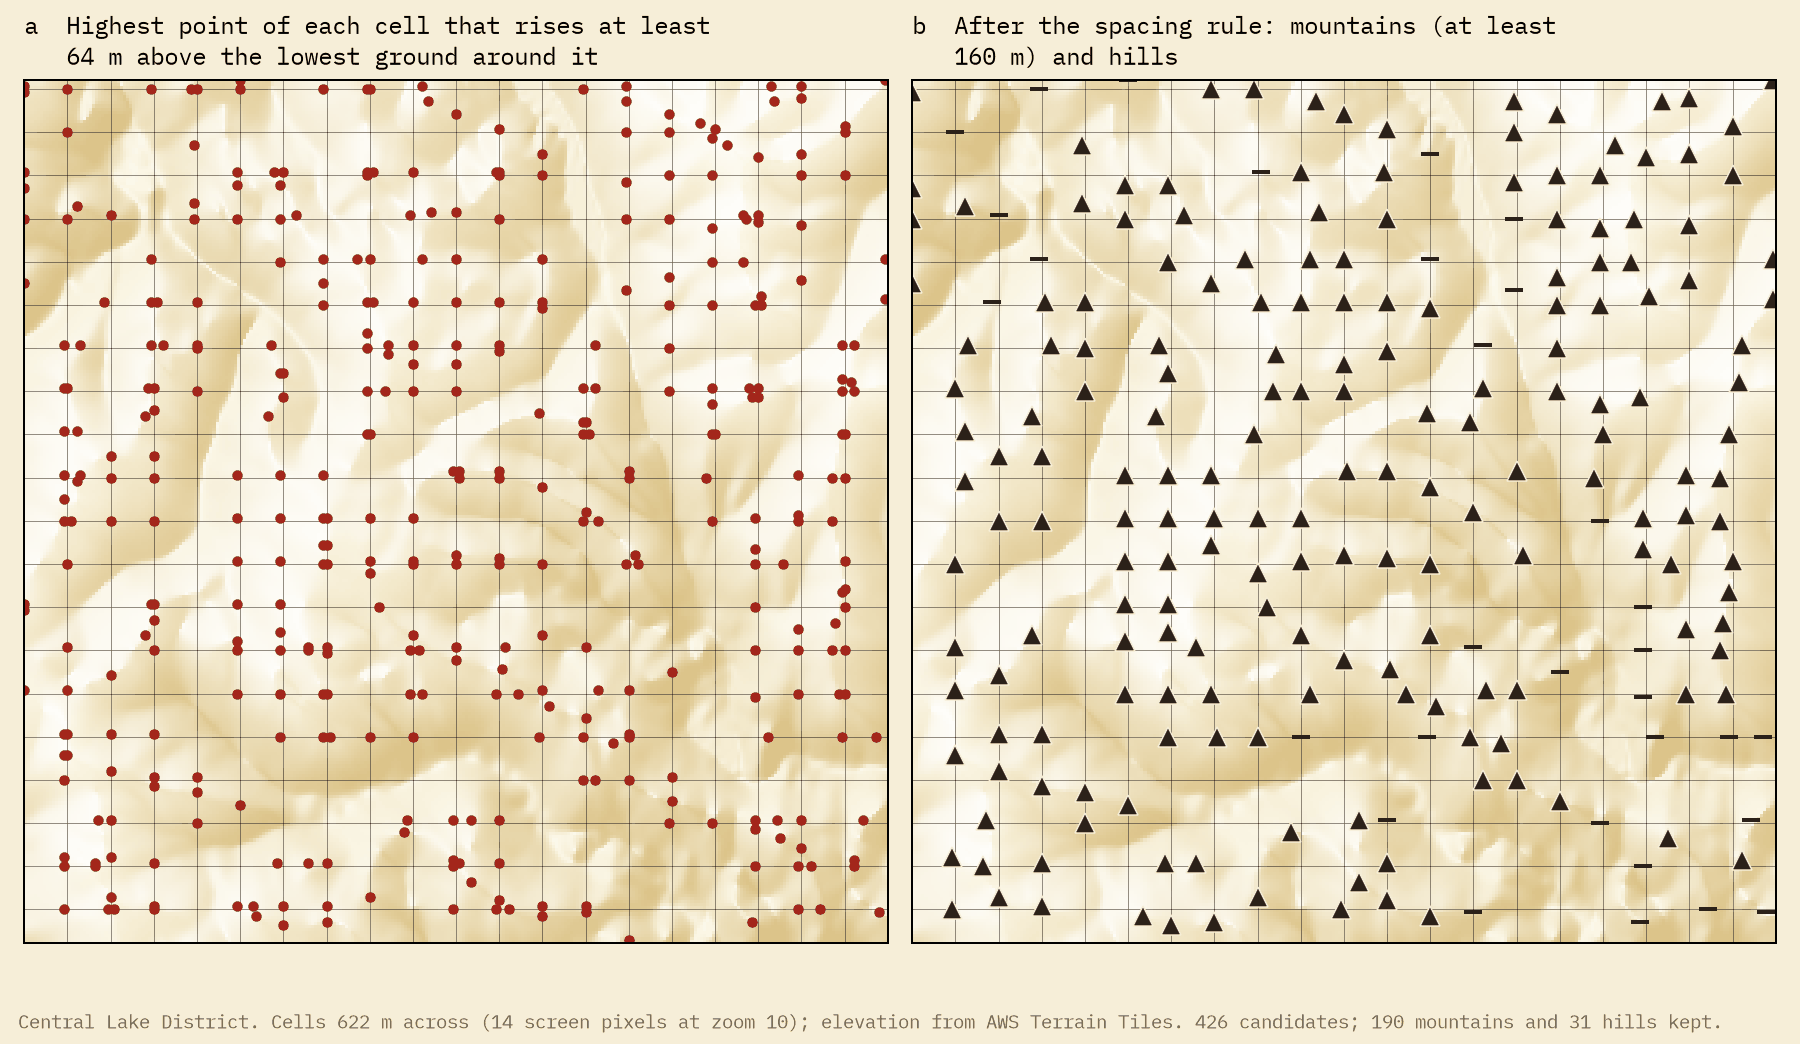
\includegraphics[width=\textwidth]{f_method.png}
\caption{The mountain rule on real elevation, central Lake District, cells of 622~m (rank 10). (a) Each cell's highest point that clears the hill bar. (b) After the spacing rule: mountains clear 160~m of relief, hills 64~m. Computed with a Python transcription of the worker's rule.}\label{fig:method}\end{figure}

\subsection{Woods, marsh and moor}
From zoom 7 the worker also reads the OpenStreetMap land cover in the vector tile for the same area and paints the woods, wetlands and heaths into small $256\times256$ masks. Tree and tuft glyphs are scattered on a nested jittered grid (cells of 10 and 20 pixels), in which a point chosen for a cell is inherited by whichever child cell contains it; points are kept where the mask is set. Woods tagged as forest get mostly conifers, other woods mostly broadleaf trees. Tufts start at zoom 9.

\subsection{Ink cap}
A rule that places a peak wherever the ground is rugged enough fills a great range or a high plateau with a solid carpet of glyphs. Hand-drawn maps leave paper between the peaks, so the worker caps the ink. Each tile is divided into $6\times6$ patches. Glyphs are taken coarsest rank first and, within a rank, mountains before hills and the most prominent first; each is sized as the style will draw it in the middle of the tile's zoom, and a mountain is kept only while the summed footprints of the mountains in its patch stay under 0.75 of the patch area, or 0.45 where the candidate mountains would ink the patch more than 1.6 times over. Hills are kept while all glyphs stay under 1.05. Taking coarse ranks first keeps the nesting: the peaks of one zoom are still the first chosen at the next. In the Lake District the cap removes fewer than one peak in ten; on a forced carpet (relief multiplied by twelve, with thinning and the ruggedness test off) it cuts 3,740 mountains to 398. On the Tibetan Plateau ecoregions the ruggedness bar is multiplied by 2.5, so that the plateau floor stays bare or in hills and only its ranges are peaked.

\subsection{Biome glyphs}
Between the ranges, glyphs on a nested jittered grid (cells of 20 pixels) take the class of the biome mask at their position: crescent dunes with sand stipple, tufts of grass, clusters of round crowns with the odd palm, small pointed conifers, pale blue hatching or crevasse lines on ice, and marsh and tundra tufts. Each class keeps a different share of the grid points, from about a sixth on the tundra to nearly all in the rainforest. OpenStreetMap glaciers count as ice and OpenStreetMap sand as desert, and biome glyphs keep clear of mountains and water. Rainforest and taiga glyphs fade out by zoom 7, where OpenStreetMap's own woods take over.

\subsection{Nothing on water}
Every glyph is checked against a mask of the OpenStreetMap \texttt{water} layer for its tile, and mountains and hills must also keep one or two mask pixels clear of the water's edge and stand on ground above sea level. This keeps seamounts, and small islands too small to show at the current zoom, from drawing a lone mountain in an empty ocean.

\subsection{Lettering}
Names are placed before glyphs and never overlap each other; glyphs then give way wherever a name sits, as a map maker would leave a gap for the lettering. Country names follow an arc fitted to each country's largest part: the principal axis of its interior gives the direction (level for round shapes, up to 50 degrees, or 80 for long thin countries), and a quadratic bow is fitted to the midpoints of cross sections, limited to a tenth of the length. For 17 countries whose shape defeats this, such as Russia, Canada, Chile, Norway and Indonesia, I drew the curve by hand. 167 further names are drawn by hand on curves: 62 uplands, lowlands and seas around Britain and Ireland, and 105 oceans, seas, ranges, deserts and regions elsewhere. Ranges are lettered along their flanks rather than their crests, so that the peaks stay visible.

MapLibre decides whether a curved name fits from the length of its line, so each curve is stored once per zoom band, cut to its central part when it is long, or drawn out a little past its ends when the name is wider than the land, and left out of bands where it would need to be drawn out too far. Text widths are measured from the font files with the same sizes and letter spacing as the style. Other names, cities, towns, villages, peaks with heights, rivers, lakes, smaller seas and national parks, come live from OpenStreetMap.

\subsection{Heritage, towns and decoration}
Heritage sites come from Wikidata \citep{wikidata} (castles, palaces, seats of government, churches, cathedrals and abbeys, monasteries, great houses, ruins, prehistoric sites, parks, natural features and World Heritage Sites), joined with data sets of architecture, tall buildings, lighthouses, battles and monasteries built from the same source. Each site is given a pictogram by its type and a first zoom $z = \max(6, 12.5 - 1.45\log_2(1 + n))$ from its number $n$ of Wikipedia articles; outside Britain and Ireland the commoner kinds need more articles. They are stored as small files on a zoom 6 grid, which the worker reads and returns as a point layer with at most 650 sites per tile, sorted by first zoom so the best known win any collision. About 150 world-famous monuments have bespoke drawings, a list of great summits (each country's and region's highest point and famous peaks) gets a larger drawing and lettering, and walls, dykes and aqueducts follow their OpenStreetMap lines. Mountains are capped with snow above a snow line that falls with latitude from 3,500~m in the tropics to sea level near the poles, and rugged ground well above it is hatched in pale blue. From zoom 12 the worker draws towns: townhouses on both sides of each street in the tile, facing it, kept with a probability that falls with distance from the place centre (scaled by a radius for each kind of place) and rises with the density of mapped buildings, on an occupancy grid so none overprint, with a market square and church at the centre and, for capitals, a wall ring. River and lake names out to zoom 9 come from Natural Earth's 1:10m rivers, lake centrelines and lakes \citep{naturalearth}, and named hills from Wikidata fill in where OpenStreetMap has no summit. Heritage names are thinned in the worker to one per cell of about 140 by 90 screen pixels, best known first, and place names outrank them in placement. Animals in their native ranges, whales at their gathering grounds, sailing ships on passages from the CLIWOC logbooks \citep{cliwoc}, the busiest airports as flying machines and a few balloons and sea serpents (marked decorative) come from a short hand-made list.

\subsection{One drawing at every zoom}
Every visual parameter is an interpolated function of zoom: glyph size and density, ink widths, the number of thin ripple lines along the coast (two far out, up to five close in), the strength of the blue wash, letter size and letter spacing. New layers fade in over a zoom or so rather than switching on. Figure~\ref{fig:zoom} shows nine zooms over the Lake District.

\section{Results}
Figures~\ref{fig:world} to~\ref{fig:lakes} show the map at several scales, with the biomes in Figures~\ref{fig:sahara} to~\ref{fig:greenland}; the renders were made from saved copies of the live tiles. At zoom 1.6 the world view draws 575 mountains and 498 hills; the view of central and South Asia at zoom 3.5 draws 1,385 mountains and 1,637 hills, and the Lake District at zoom 11 draws 1,184 mountains, 2,126 hills, 1,702 trees and 6,933 tufts. As a stress test for the great ranges, which the saved tiles did not cover at high zoom, Figure~\ref{fig:stress} multiplies the Lake District's relief by six, giving a range as steep, cell for cell, as the high Himalaya at zoom 8.

\begin{figure}[tbp]\centering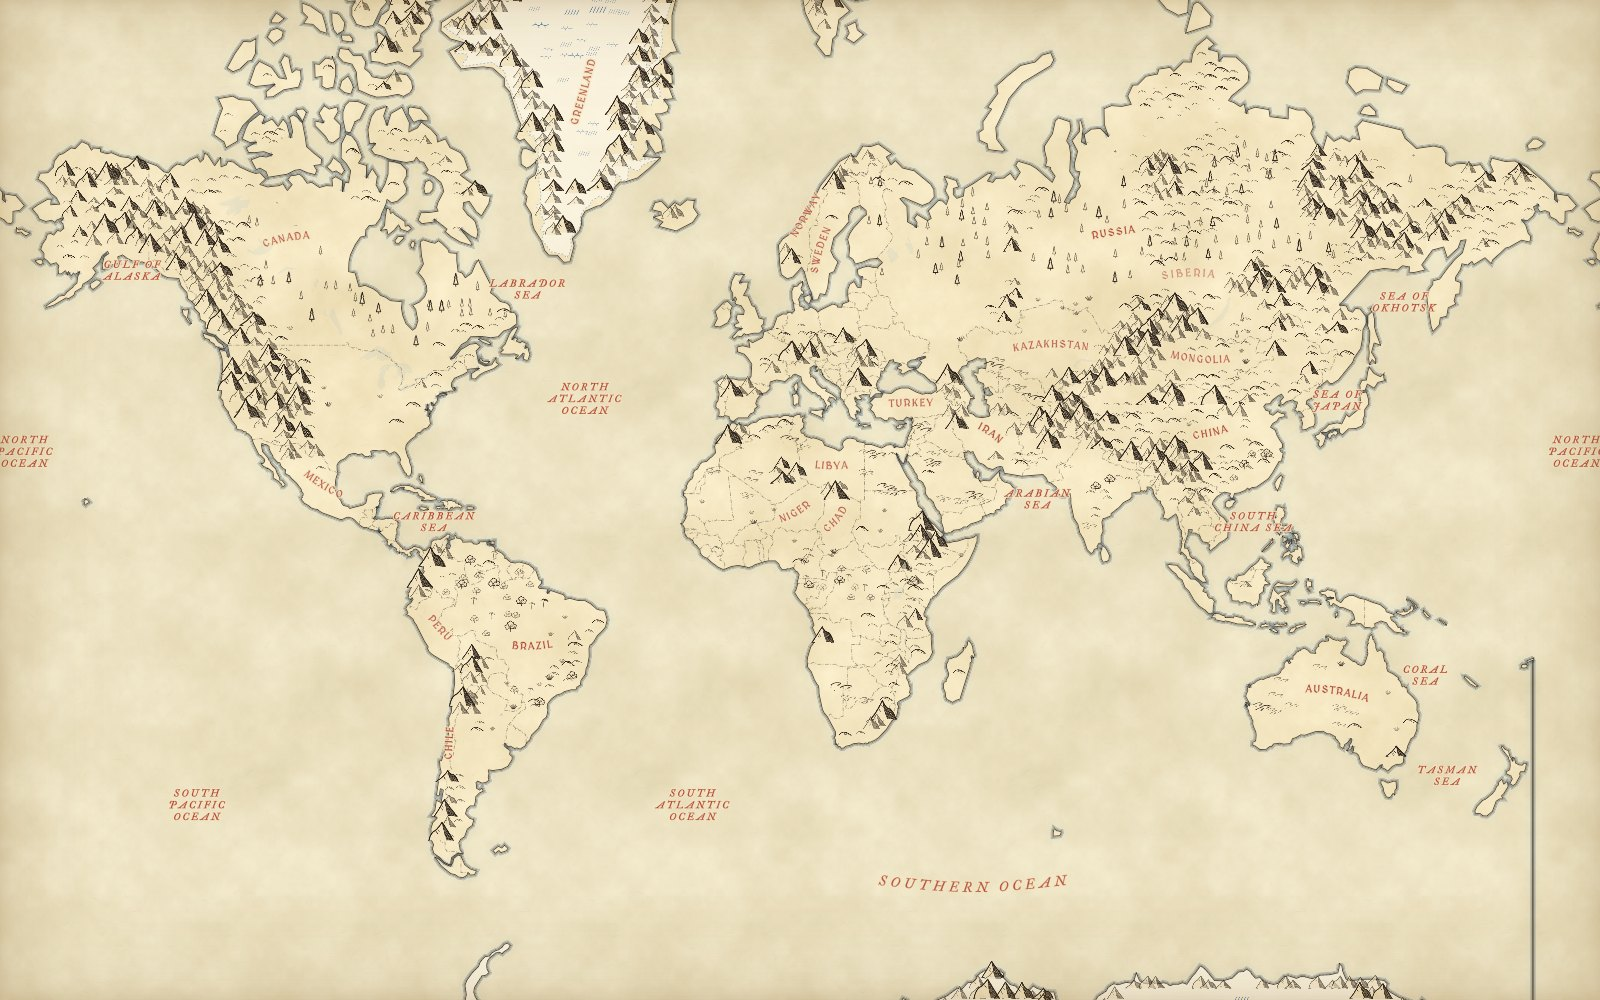
\includegraphics[width=\textwidth]{f_world.jpg}
\caption{The whole world at zoom 1.6.}\label{fig:world}\end{figure}
\begin{figure}[tbp]\centering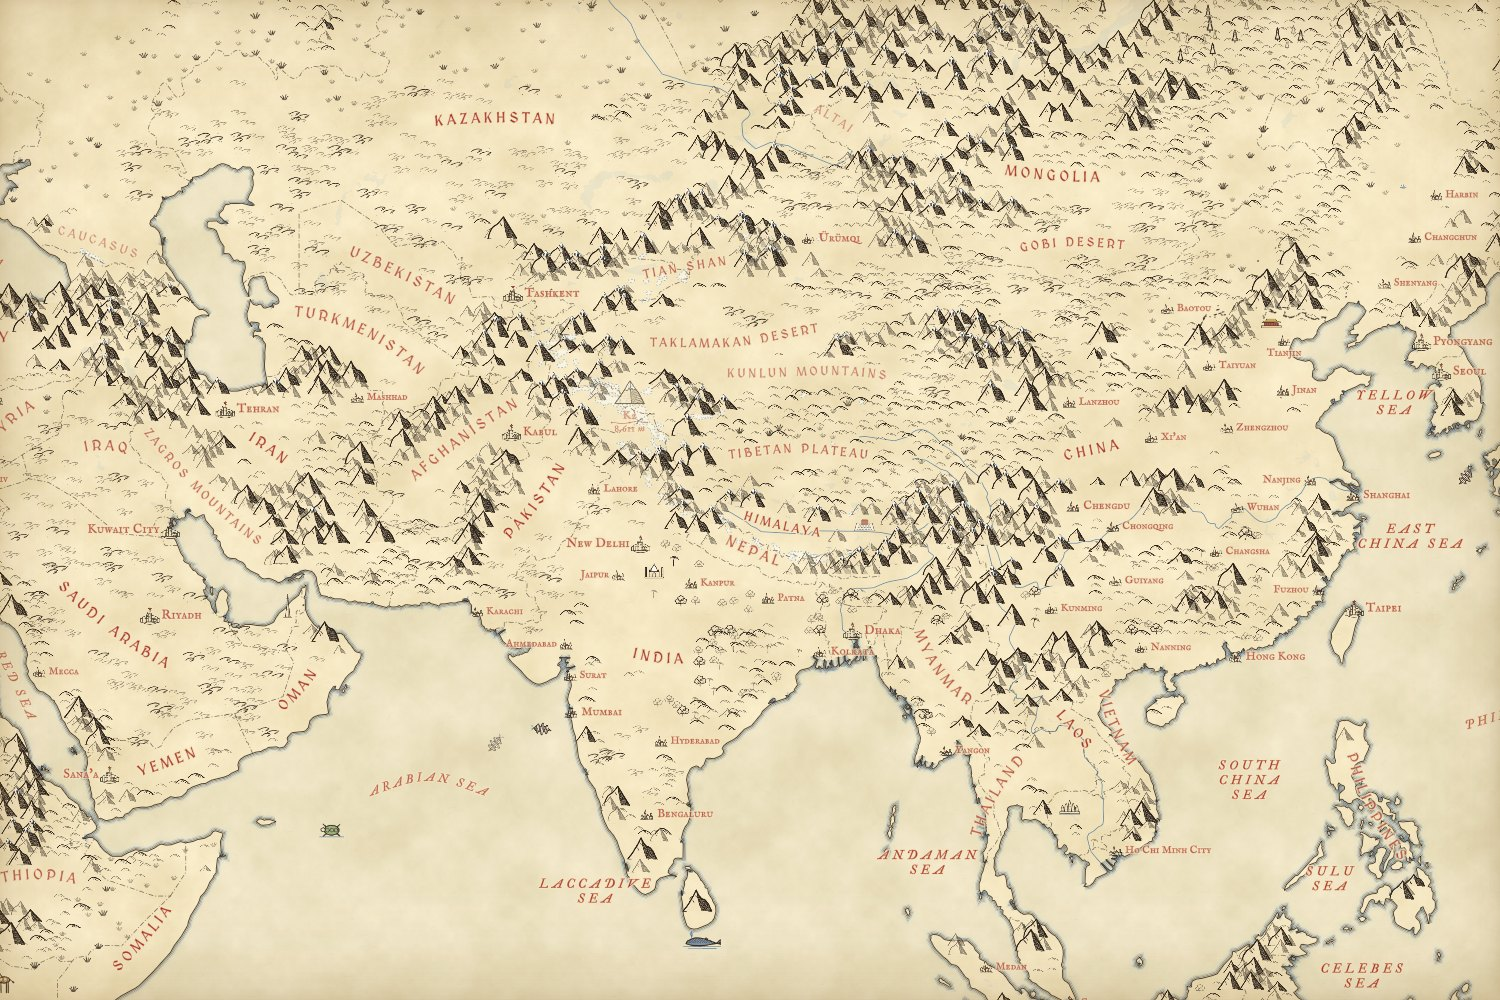
\includegraphics[width=\textwidth]{f_asia.jpg}
\caption{Central and South Asia at zoom 3.5: the Himalaya, Tibetan Plateau, Tian Shan and Kunlun lettered on curves.}\label{fig:asia}\end{figure}
\begin{figure}[tbp]\centering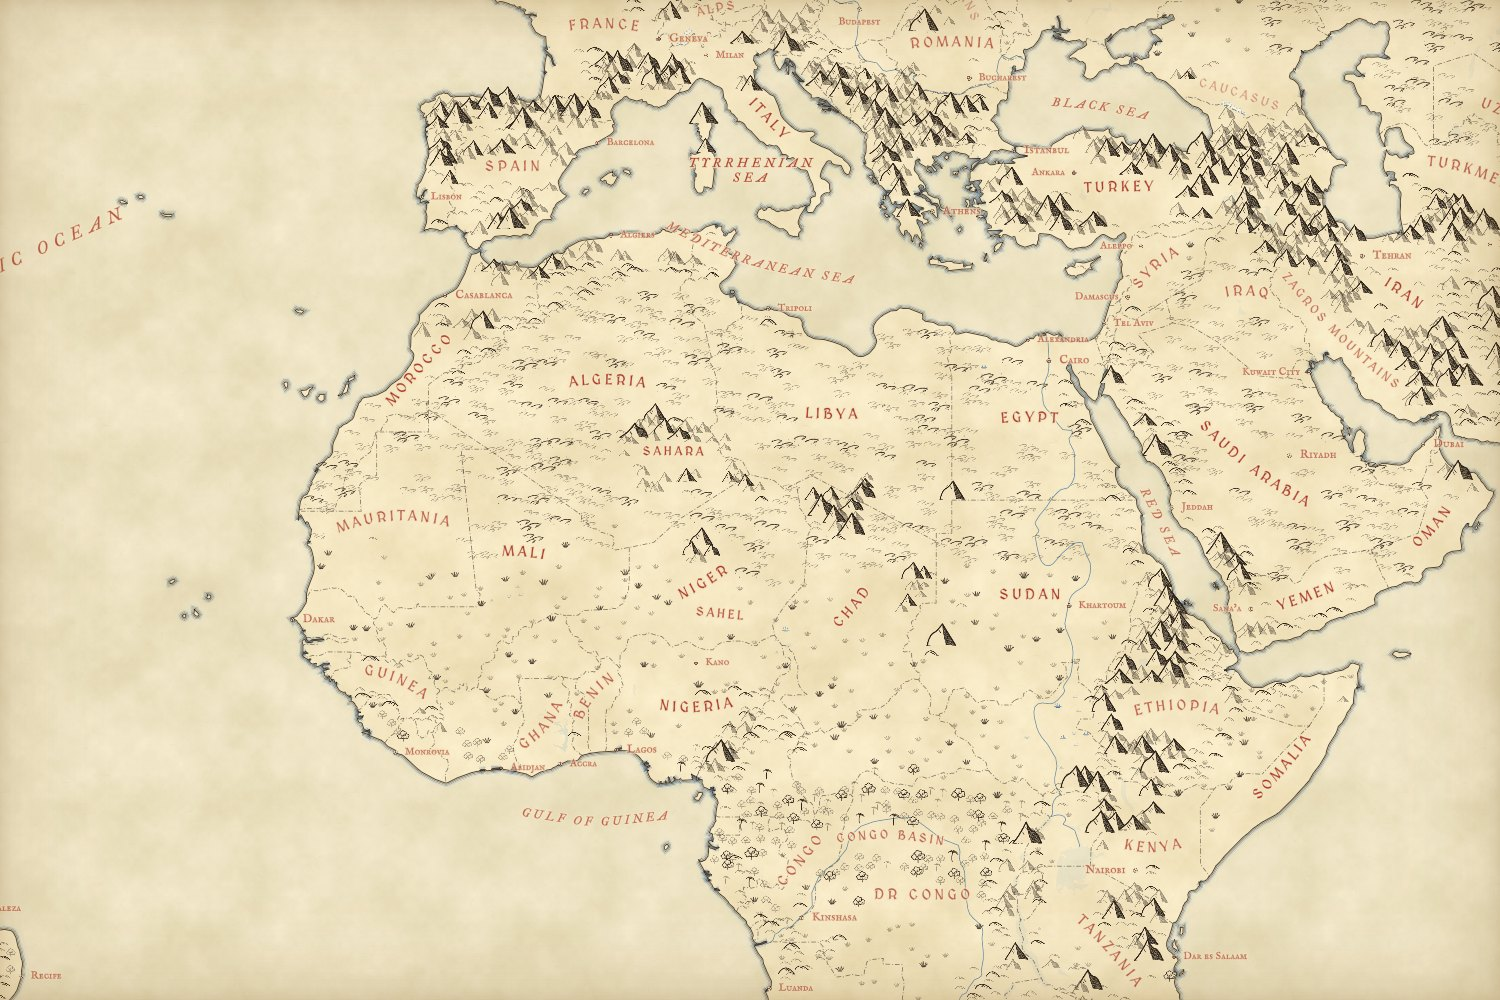
\includegraphics[width=\textwidth]{f_sahara.jpg}
\caption{The Sahara at zoom 3.45: dunes across the desert, peaks only on the Atlas, the Ahaggar, the Tibesti and the highlands round it, steppe tufts in the Sahel and rainforest crowns along the Gulf of Guinea.}\label{fig:sahara}\end{figure}
\begin{figure}[tbp]\centering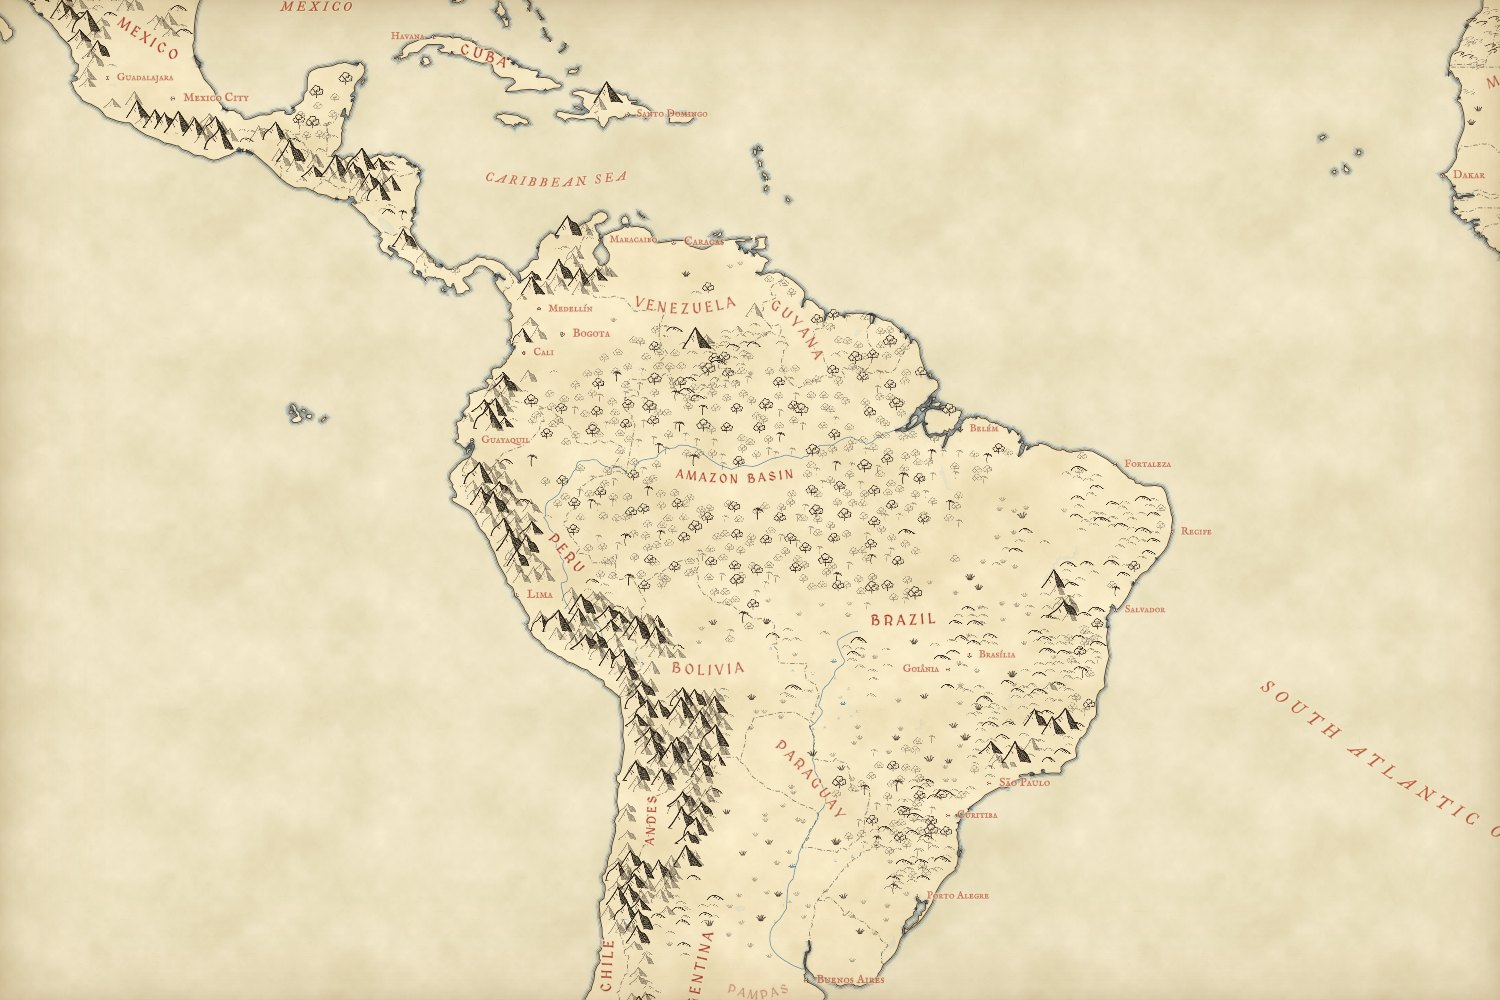
\includegraphics[width=\textwidth]{f_amazon.jpg}
\caption{The Amazon at zoom 3.45: rainforest crowns and palms, with the Andes to the west.}\label{fig:amazon}\end{figure}
\begin{figure}[tbp]\centering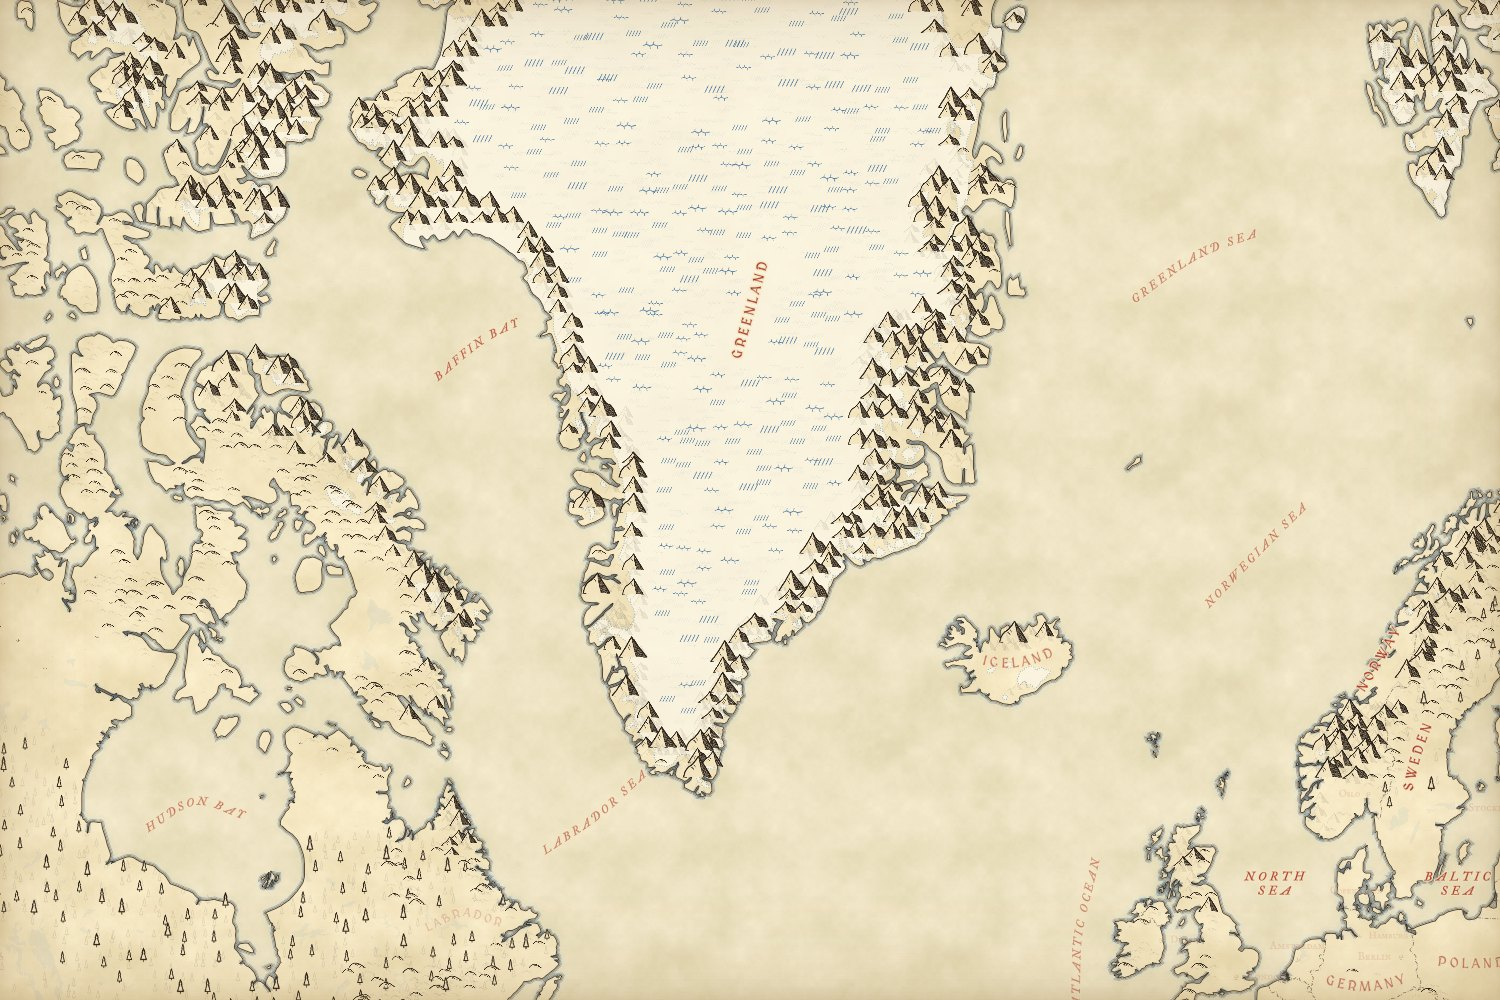
\includegraphics[width=\textwidth]{f_greenland.jpg}
\caption{Greenland at zoom 3.1: blue hatching and crevasse lines on the ice sheet, mountains only on the rugged coasts.}\label{fig:greenland}\end{figure}
\begin{figure}[tbp]\centering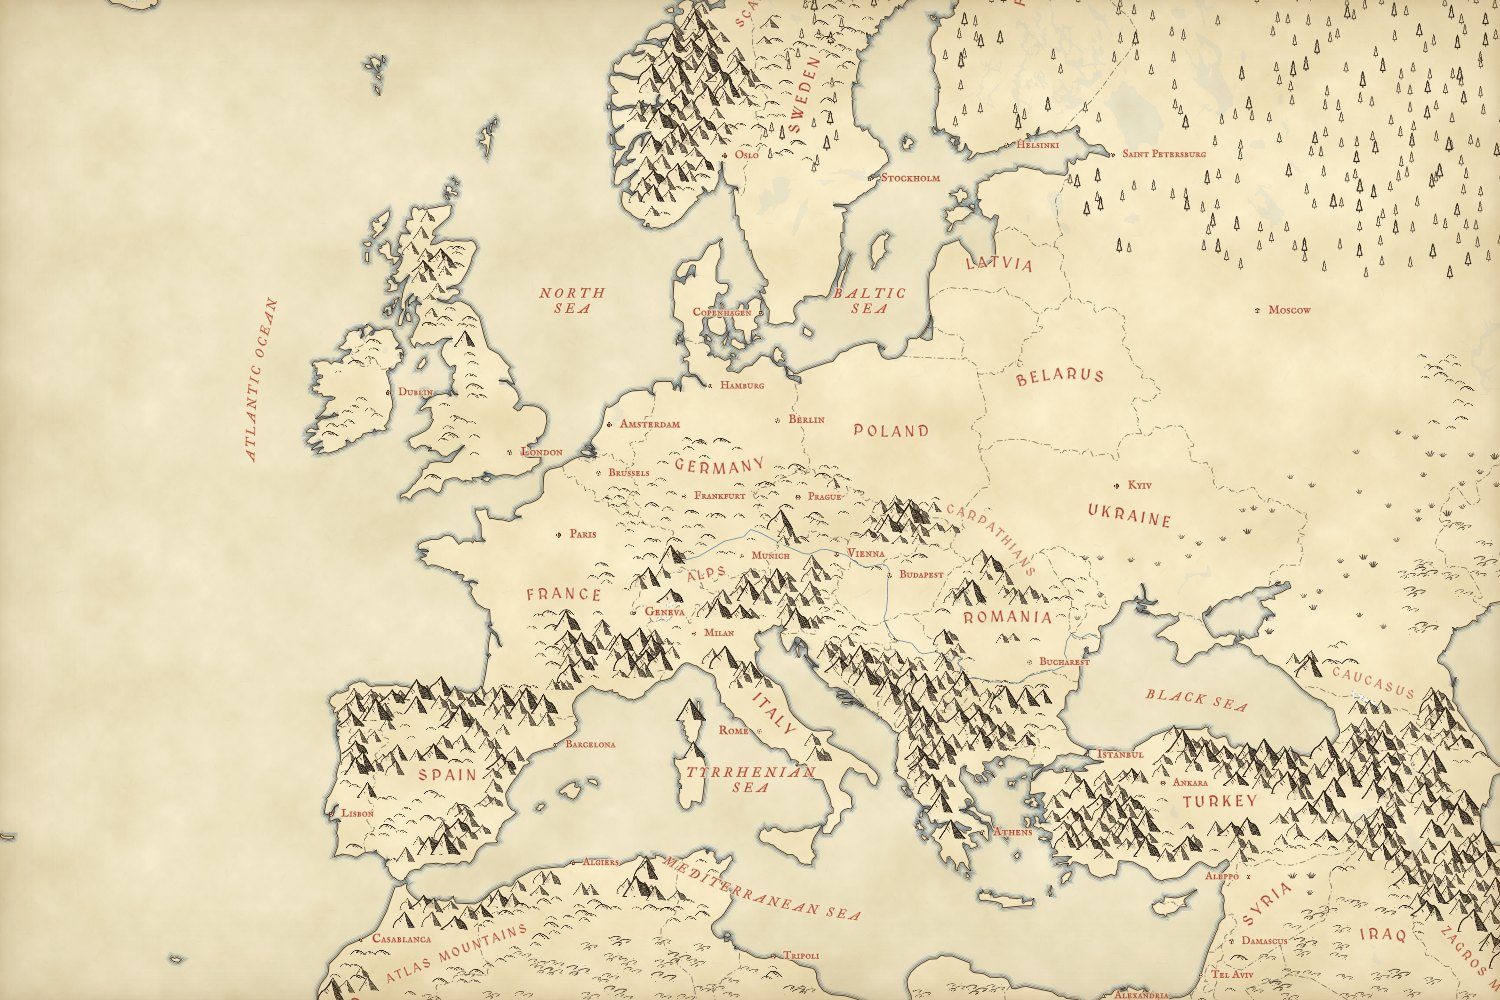
\includegraphics[width=\textwidth]{f_europe.jpg}
\caption{Europe at zoom 3.8.}\label{fig:europe}\end{figure}
\begin{figure}[tbp]\centering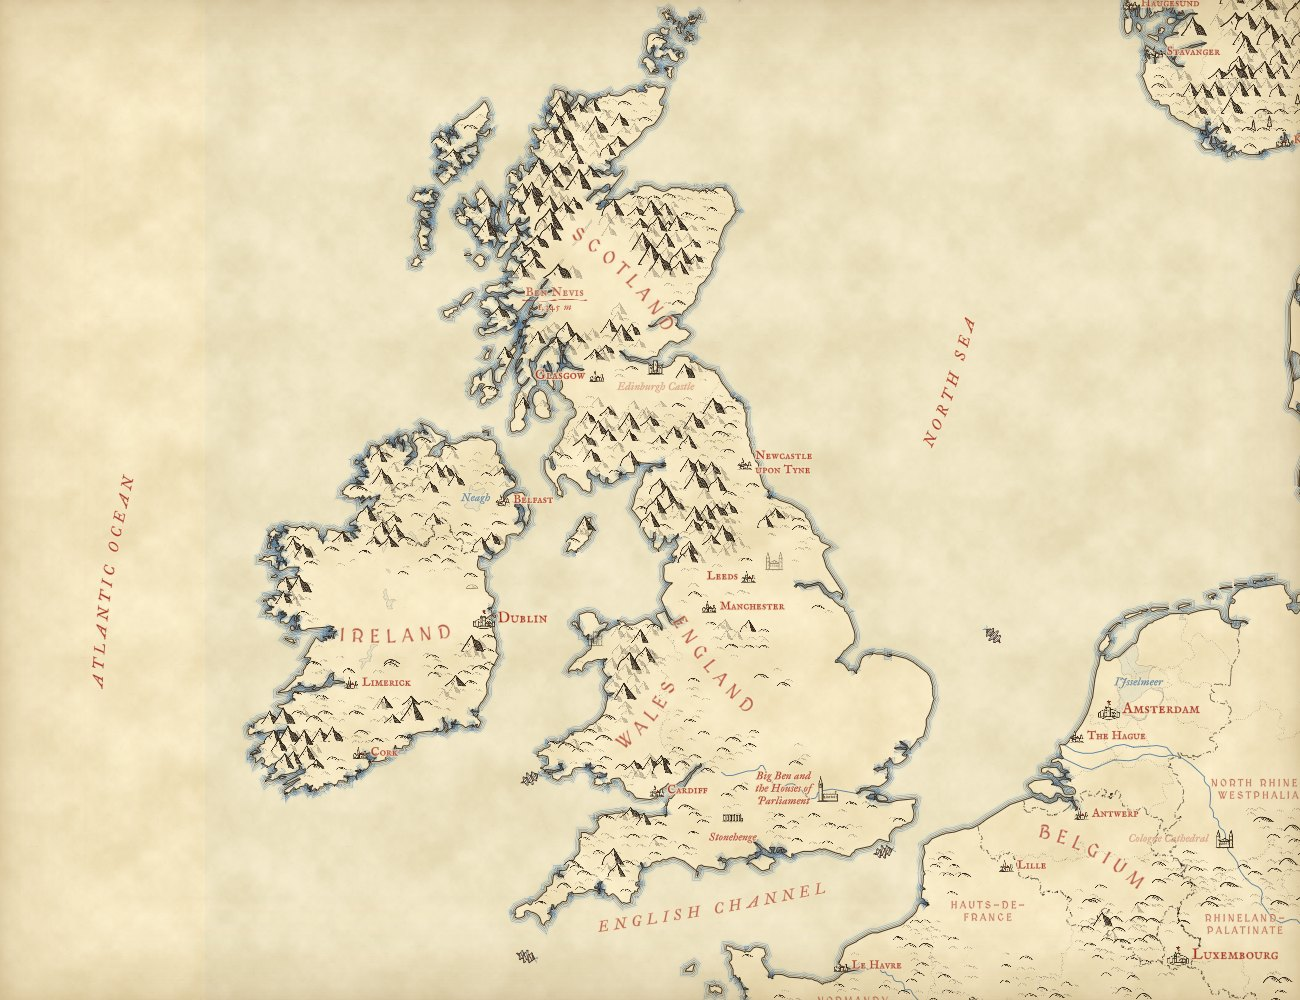
\includegraphics[width=0.85\textwidth]{f_gb.jpg}
\caption{Britain and Ireland at zoom 5.3.}\label{fig:gb}\end{figure}
\begin{figure}[tbp]\centering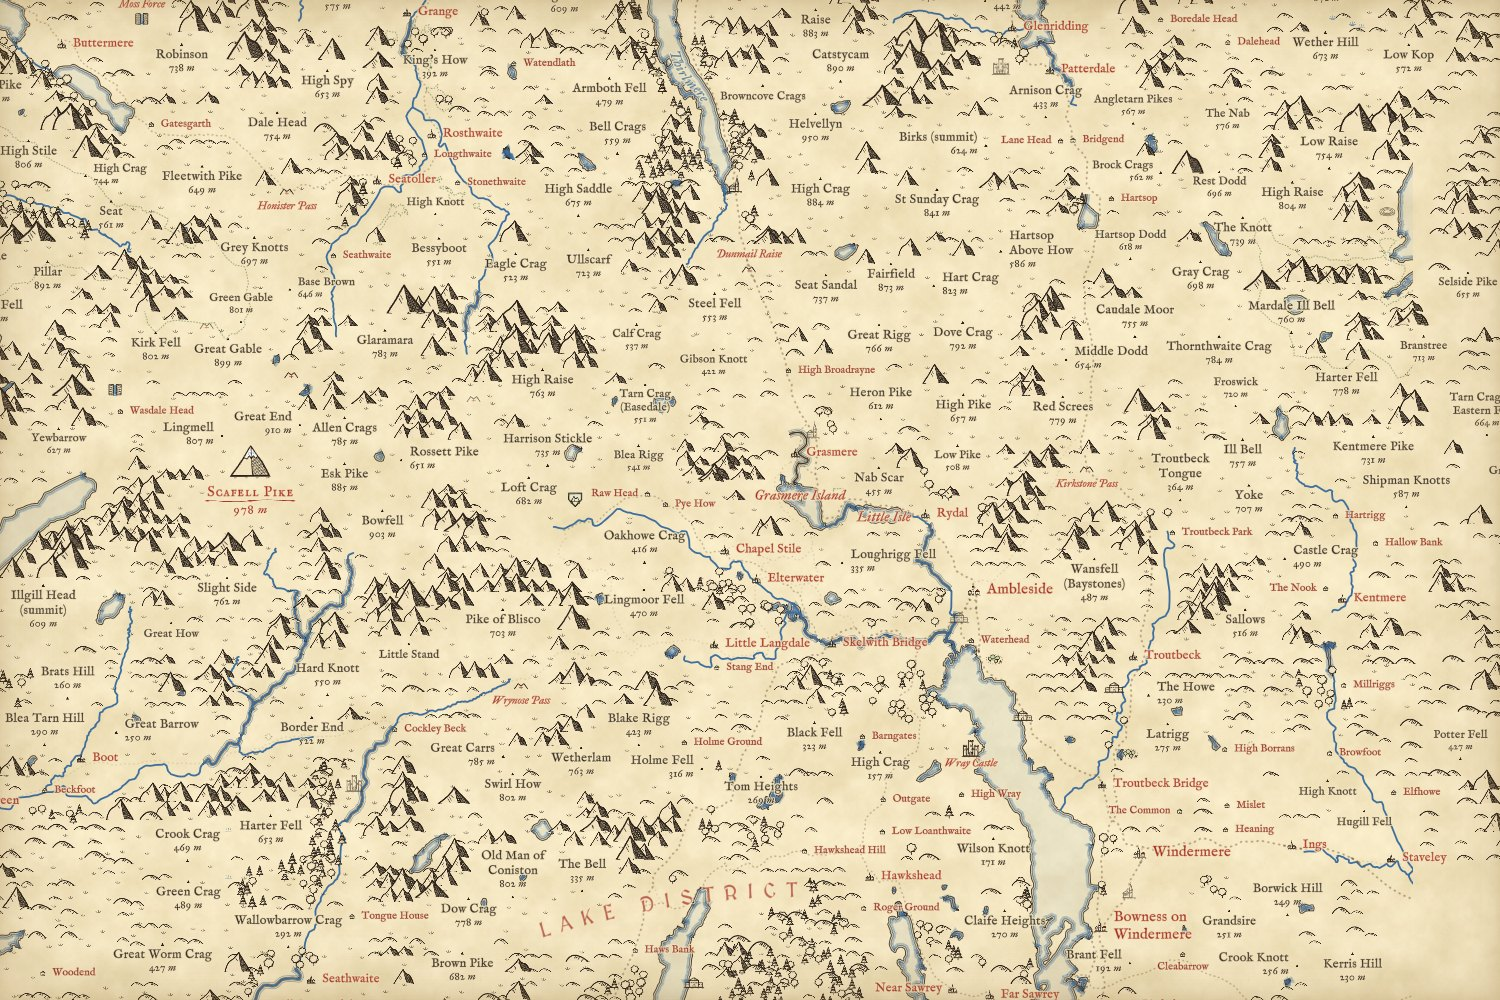
\includegraphics[width=\textwidth]{f_lakes.jpg}
\caption{The central Lake District at zoom 11: fells with their heights, villages, woods and moorland.}\label{fig:lakes}\end{figure}
\begin{figure}[tbp]\centering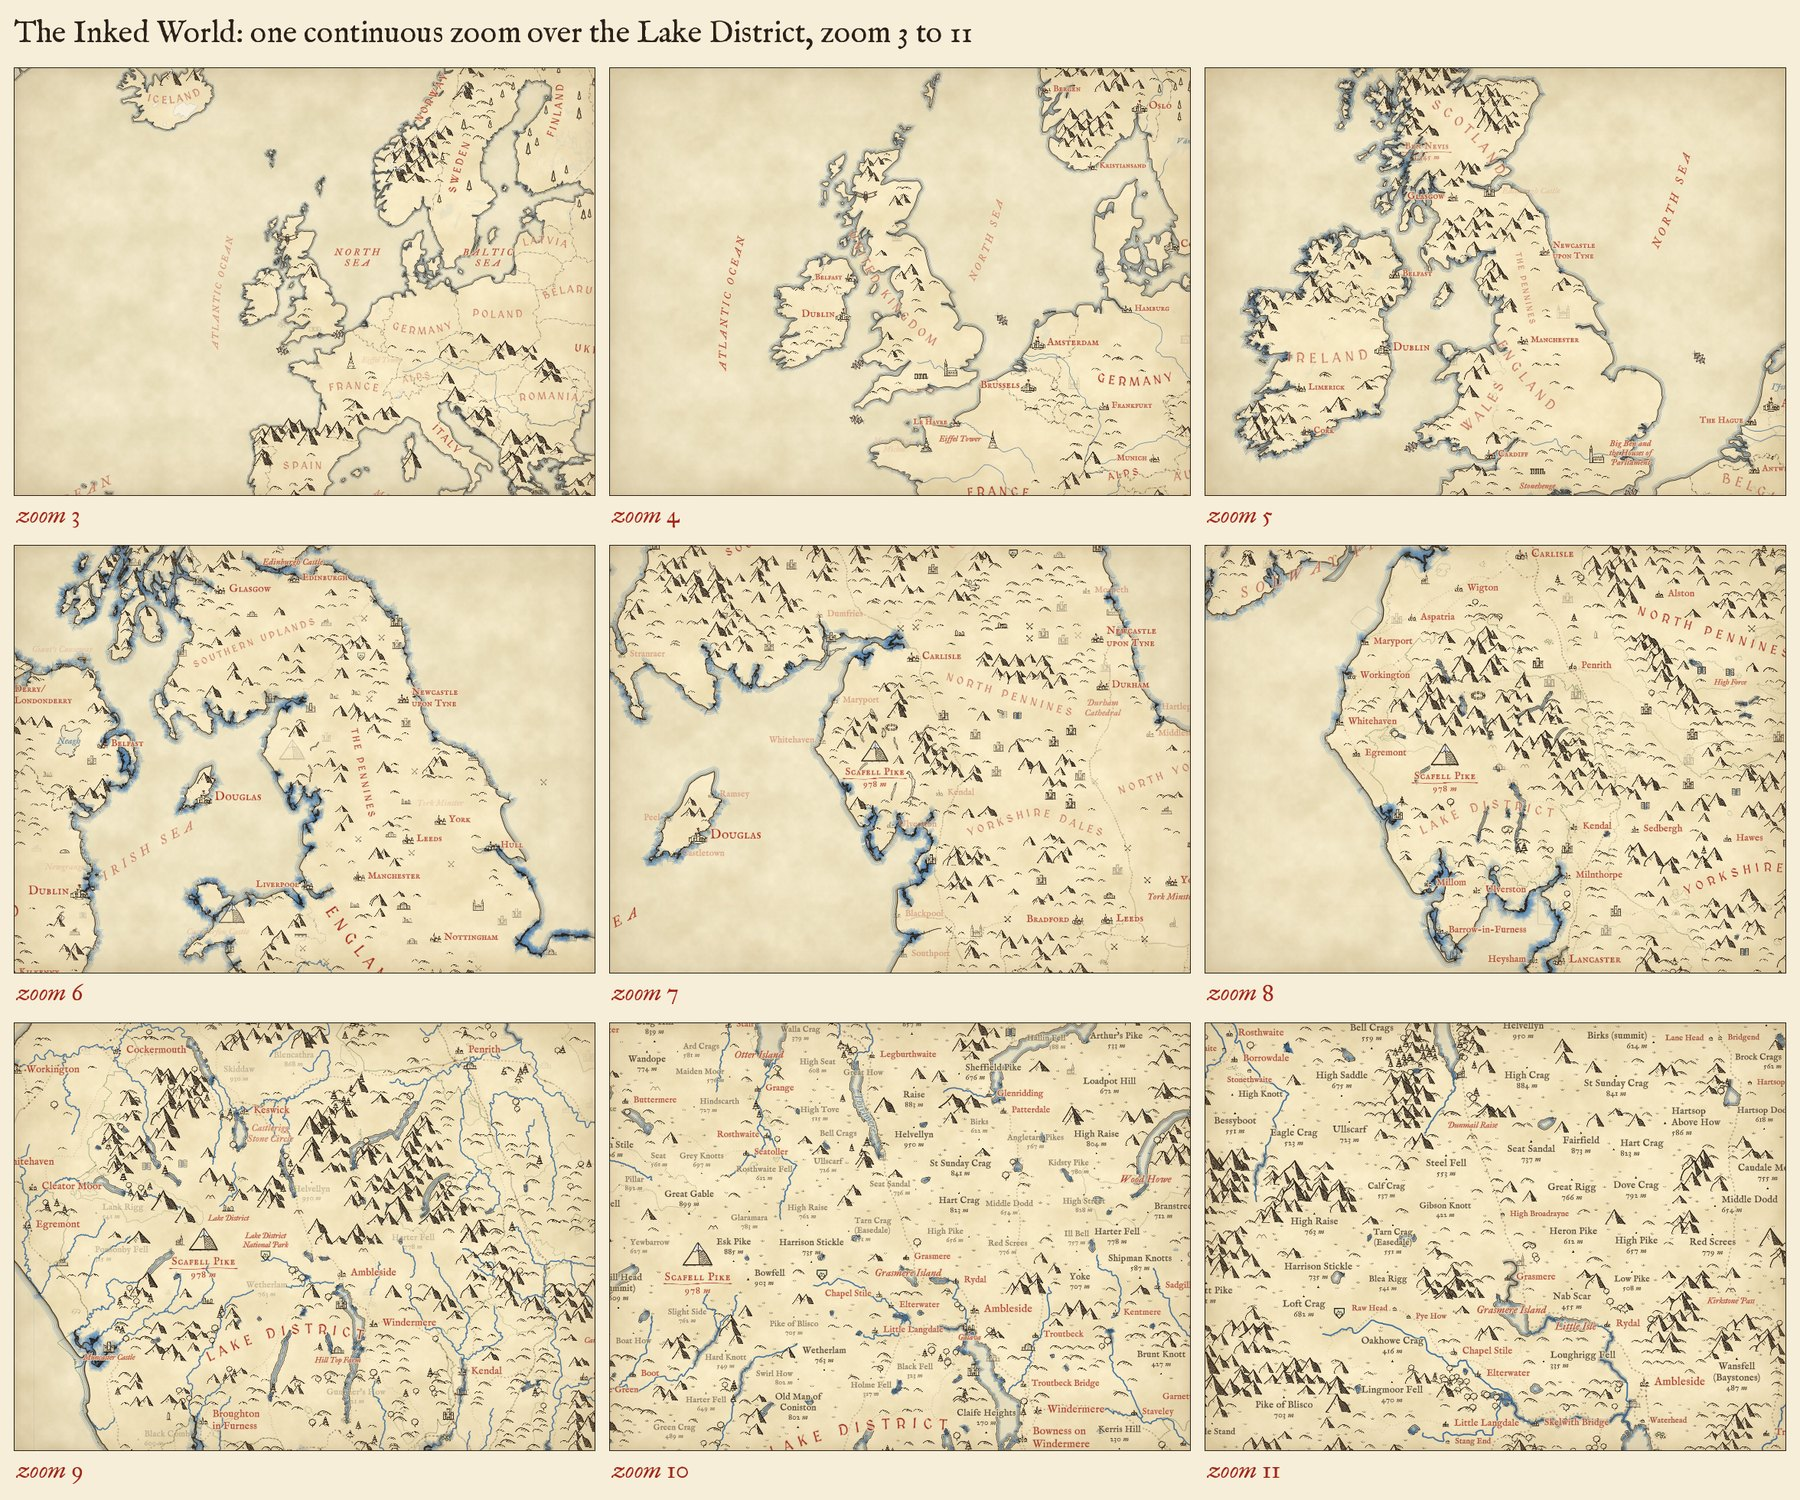
\includegraphics[width=\textwidth]{f_zoom.jpg}
\caption{One continuous zoom over the Lake District, zoom 3 to 11.}\label{fig:zoom}\end{figure}
\begin{figure}[tbp]\centering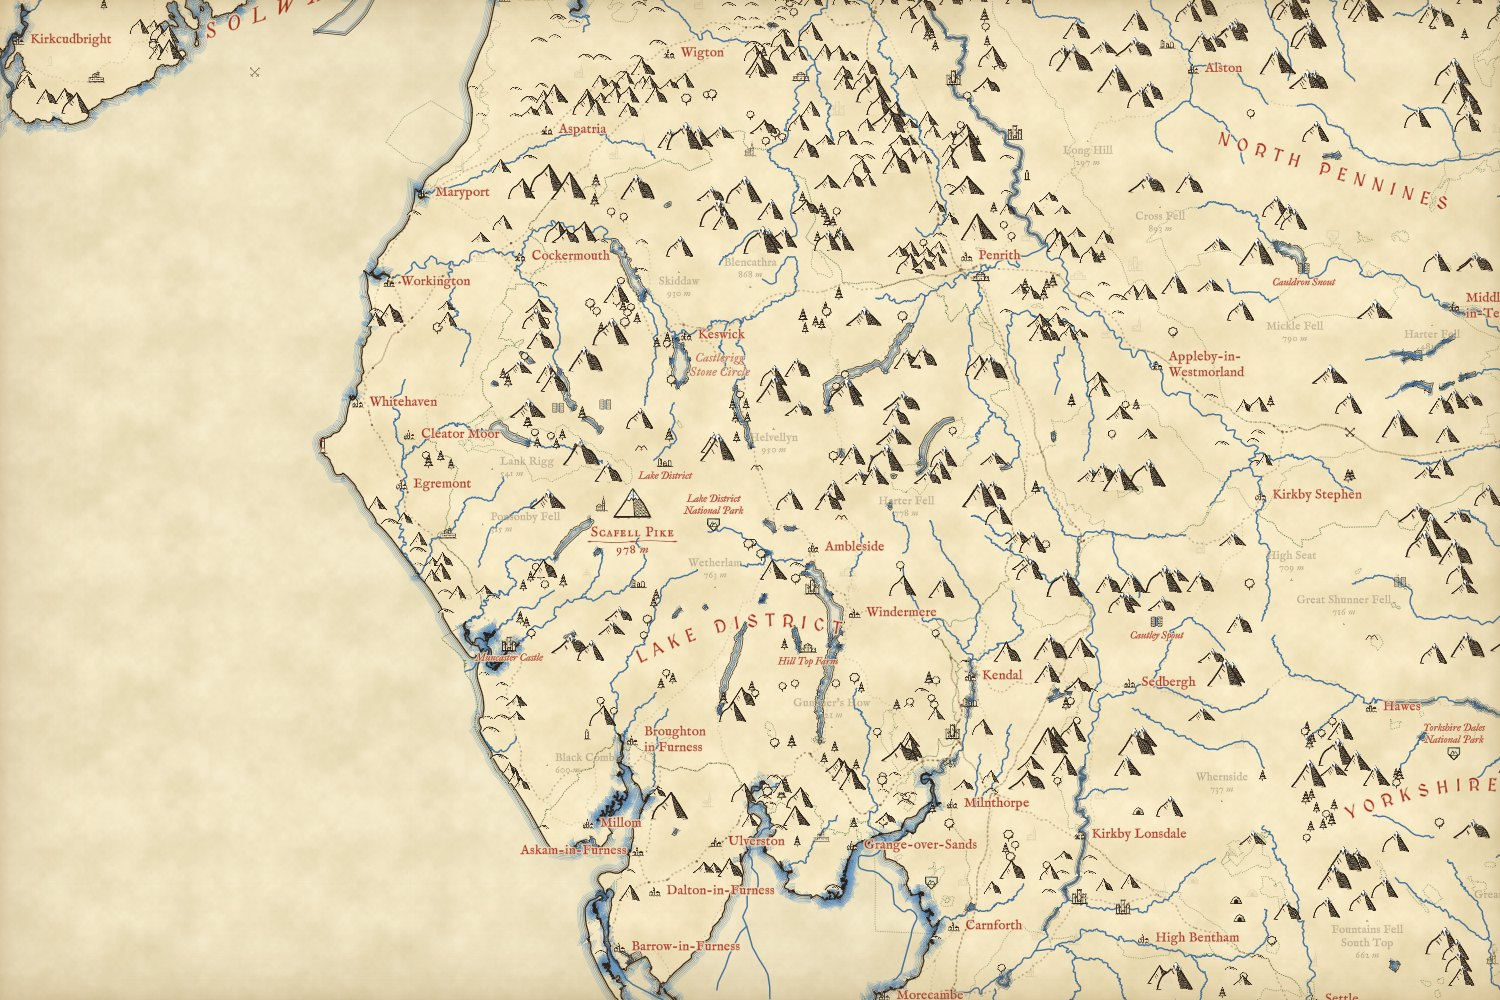
\includegraphics[width=\textwidth]{f_stress.jpg}
\caption{Stress test: the Lake District at zoom 9 with its relief multiplied by six, a stand-in for a great range. The thinning rule keeps ridges and summits apart.}\label{fig:stress}\end{figure}

\section{Checks}
The container in which the map was built could not reach the tile services, so it was developed against saved tiles: OpenFreeMap tiles for the world at zoom 0 to 3, the United Kingdom at 4 to 8 and the Lake District and North Yorkshire at 9 to 12, and Terrain Tiles for the same areas. Screenshots of every change were taken with Playwright and compared by eye. A live check page in the repository (\texttt{qa\_live/}) steps one map through a list of views in the Alps, the Himalaya, the Rockies, the Andes, the Sahara, Japan, New Zealand and the Norwegian fjords and records a snapshot and glyph counts for each, for review in a browser once the page is published. The style is validated against the MapLibre style specification.

\section{Limitations}
First, peaks are placed on the highest point of grid cells, not on named summits, and their size shows local relief, not height; a named peak and its glyph may sit a little apart. Second, the threshold and thinning were tuned by eye in Britain and checked elsewhere at low zoom and with the stress test above; some ranges may look denser or sparser than a map maker would draw them. Third, the ruggedness bars, the montane and open-biome factors and the biome mask were tuned on coarse world tiles and on Britain; the biome mask is coarse and its montane flag comes from names. Fourth, woods appear only from zoom 7, because the tiles carry no land cover further out, and they are only as complete as OpenStreetMap. Fifth, the hand-placed names are my choice and their curves my drawing; elsewhere names are OpenStreetMap's, and smaller seas and regions are lettered straight. Sixth, the glyphs are computed in the browser, so a new area takes a second or two to draw, and very old browsers without workers that can draw on canvas show the map without glyphs. Finally, the look is a style, not a historical reconstruction: it borrows the conventions of hand-drawn maps without claiming their authority.

\section{Conclusion}
A small set of drawing rules, applied to open elevation and OpenStreetMap data in the reader's browser, is enough to give the whole world the look of a hand-inked map, and to keep that look as one zooms from continents to single hills. The rules are simple: highest points of nested cells, a relief bar that grows with the size of a cell, a little spacing and thinning, masks for woods and water, and names placed first.

\section*{Data and code availability}
The interactive map is at \url{https://maps.tristanhotham.com/ink-map/}. Code and the derived label files are at \url{https://github.com/Tristan-Hotham/ink-map} and archived with this paper at \url{https://doi.org/10.5281/zenodo.23860253}. Code is under the MIT licence; text, figures and derived files under CC BY 4.0. The map shows OpenStreetMap data, \textcopyright{} OpenStreetMap contributors, under the Open Database Licence; figures that show it carry that credit. Fonts are under the SIL Open Font License.

\section*{AI statement}
I wrote the text, with drafting and editing assistance from Claude (Anthropic), which also helped prepare the analysis code. I reviewed and checked all text and results.

\begin{thebibliography}{9}
\bibitem[Google Fonts(2026)]{fonts} Google Fonts (2026) MedievalSharp (wmk69) and IM Fell types (Igino Marini). SIL Open Font License 1.1. \url{https://github.com/google/fonts}
\bibitem[Dinerstein et al.(2017)]{resolve} Dinerstein, E., Olson, D., Joshi, A. et al. (2017) An ecoregion-based approach to protecting half the terrestrial realm. \emph{BioScience} 67(6), 534 to 545. \url{https://doi.org/10.1093/biosci/bix014}. Data: RESOLVE Ecoregions 2017, CC BY 4.0, \url{https://ecoregions.appspot.com/}
\bibitem[Garc\'ia-Herrera et al.(2005)]{cliwoc} Garc\'ia-Herrera, R., K\"onnen, G. P., Wheeler, D. A. et al. (2005) CLIWOC: a climatological database for the world's oceans 1750 to 1854. Climatic Change 73, 1 to 12.
\bibitem[MapLibre(2026)]{maplibre} MapLibre contributors (2026) MapLibre GL JS 4.7. BSD 3-Clause. \url{https://maplibre.org/}
\bibitem[Natural Earth(2026)]{naturalearth} Natural Earth (2026) Admin 0 countries, populated places, admin 1 states and provinces. Public domain. \url{https://www.naturalearthdata.com/}
\bibitem[ONS(2023)]{ons} Office for National Statistics (2023) Local Authority Districts, boundaries. Open Government Licence v3.0. \url{https://geoportal.statistics.gov.uk/}
\bibitem[OpenFreeMap(2026)]{openfreemap} OpenFreeMap (2026) Free vector map tiles. \url{https://openfreemap.org/}
\bibitem[OpenMapTiles(2026)]{openmaptiles} OpenMapTiles (2026) Vector tile schema. \url{https://openmaptiles.org/schema/}
\bibitem[OpenStreetMap(2026)]{osm} OpenStreetMap contributors (2026) OpenStreetMap. Open Database Licence 1.0. \url{https://www.openstreetmap.org/copyright}
\bibitem[Wikidata(2026)]{wikidata} Wikidata contributors (2026) Wikidata. CC0. \url{https://www.wikidata.org/}
\bibitem[Terrain Tiles(2026)]{terrain} Mapzen and Amazon Web Services (2026) Terrain Tiles, Registry of Open Data on AWS. \url{https://registry.opendata.aws/terrain-tiles/}
\end{thebibliography}
\end{document}
